\documentclass[a4paper,12pt]{article}
\usepackage[top=2cm, bottom=2cm, left=2cm, right=2cm]{geometry}
\usepackage[utf8]{inputenc}
\usepackage{amsmath, amsfonts, amssymb}
\usepackage{graphicx}
\usepackage{float}
\usepackage{dsfont}
\usepackage[brazil]{babel}
\usepackage{indentfirst}
\usepackage{listings}
\usepackage{hyperref}
\DeclareMathOperator{\sen}{sen}
\DeclareMathOperator{\tg}{tg}
\DeclareMathOperator{\cossec}{cossec}
\DeclareMathOperator{\senh}{senh}
\DeclareMathOperator{\tgh}{tgh}
\DeclareMathOperator{\cossech}{cossech}
\DeclareMathOperator{\arcsen}{arcsen}
\DeclareMathOperator{\arctg}{arctg}
\DeclareMathOperator{\arccossec}{arccossec}
\newcommand{\limite}{\displaystyle\lim}
\newcommand{\integral}{\displaystyle\int}
\newcommand{\soma}{\displaystyle\sum}
\newcommand{\arr}{\begin{array}}
\newcommand{\farr}{\end{array}}
\newcommand{\eq}{\begin{equation}}
\newcommand{\feq}{\end{equation}}
\newcommand{\eqn}{\begin{eqnarray*}}
\newcommand{\feqn}{\end{eqnarray*}}
\title{\textbf{Um estudo sobre o Potencial de Hénon-Heiles}}
\author{Geovanni Fernandes Garcia, N$^o$ USP: 11298560}

\usepackage{xcolor}
%\pagecolor[rgb]{0.15,0.15,0.15}
%\color[rgb]{1,1,1}


\definecolor{codegreen}{rgb}{0,0.6,0}
\definecolor{codegray}{rgb}{0.5,0.5,0.5}
\definecolor{codepurple}{rgb}{0.58,0,0.82}
\definecolor{backcolour}{rgb}{0.95,0.95,0.92}

\lstdefinestyle{mystyle}{
    backgroundcolor=\color{backcolour},   
    commentstyle=\color{codegreen},
    keywordstyle=\color{blue},
    numberstyle=\tiny\color{codegray},
    stringstyle=\color{codepurple},
    basicstyle=\ttfamily\footnotesize,
    breakatwhitespace=false,         
    breaklines=true,                 
    captionpos=b,                    
    keepspaces=true,                 
    numbers=left,                    
    numbersep=5pt,                  
    showspaces=false,                
    showstringspaces=false,
    showtabs=false,                  
    tabsize=2
}

\lstset{style=mystyle}

\begin{document}
\maketitle

Este trabalho refere-se à função Hamiltoniana apresentada por Hénon e Heiles. A Hamiltoniana de Hénon-Heiles é descrita pela expressão:

$$H = \dfrac{1}{2}(p_1^2+p_2^2+q_1^2+q_2^2) + q_1^2q_2 - \dfrac{1}{3}q_2^3$$

Essa Hamiltoniana tem sido amplamente utilizada na modelagem de sistemas astrofísicos, como estrelas binárias e núcleos galácticos, ajudando a compreender as órbitas e as interações complexas entre os corpos celestes. Além disso, a Hamiltoniana de Hénon-Heiles também tem sido aplicada no estudo de fenômenos caóticos e em sistemas moleculares, fornecendo uma visão valiosa sobre as propriedades dinâmicas e estruturais desses sistemas. O estudo e a análise da Hamiltoniana de Hénon-Heiles são essenciais para explorar as características fundamentais dos sistemas físicos não lineares e compreender os fenômenos complexos que podem surgir nesses sistemas.

Neste estudo, será construído seções de Poincaré para a Hamiltoniana de Hénon-Heiles, que é uma representação gráfica útil para sistemas Hamiltonianos com vários graus de liberdade. O cálculo numérico das seções de Poincaré consiste em duas etapas. Primeiro, precisamos de um método de integração temporal para obter as trajetórias do sistema dinâmico a partir de diferentes condições iniciais. Utilizaremos o método de Euler simplético para realizar essa primeira etapa. A segunda etapa envolve a detecção e o cálculo das interseções entre as trajetórias e uma superfície $\Sigma$, que define a seção específica do espaço de fase. Para realizar essa análise, utilizaremos o método de Hénon para avaliar numericamente essas interseções.

Inicialmente, foi implementado computacionalmente o método de Euler simplético para a Hamiltoniana de Hénon-Heiles. Em seguida, foi feito um programa em Python para construir seções de Poincaré no plano $p_2\times q_2$, considerando $q_1 = 0$ e $p_1 \geq 0$. Sugiro a leitura do código em Python detalhadamente comentado onde os gráficos deste trabalho foram produzidos, ele se encontra no link:

\url{https://colab.research.google.com/drive/10ZrmA7tqH1IjURp8mGN9pZbLaU901eE8?usp=sharing}.

A seguir, será apresentado uma descrição detalhada de cada gráfico plotado neste código, abordando seus elementos, significados e implicações.

\begin{figure}[H]
\centering
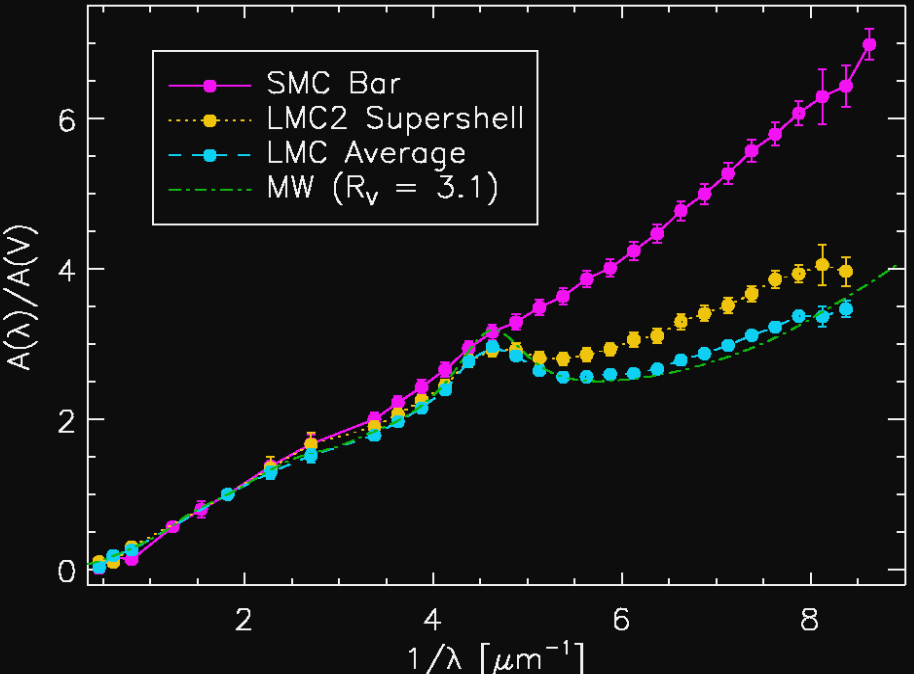
\includegraphics[width=0.72\textwidth]{grafico1.png}
\caption{\textbf{Mapas de Poincaré com interseção em $q_1 = 0$ com $E = 0,08333$.}}
\end{figure}

Na Figura 1, são apresentados quatro mapas de Poincaré com a interseção ocorrendo em $q_1 = 0$. Cada mapa é representado por pontos no plano cartesiano, com o eixo $x$ representando a variável $q_2$ e o eixo $y$ representando a variável $p_2$. Esses mapas foram gerados com diferentes valores iniciais das variáveis $q_1$ e $q_2$.

Os pontos no gráfico representam os estados das variáveis $q_2$ e $p_2$ em momentos específicos, quando $q_1$ atinge o valor de interseção ($q_1 = 0$). A cor dos pontos varia para diferenciar os diferentes mapas. Esses mapas de Poincaré são úteis para visualizar as trajetórias no espaço de fase e identificar regiões com comportamento regular ou caótico.


\begin{figure}[H]
\centering
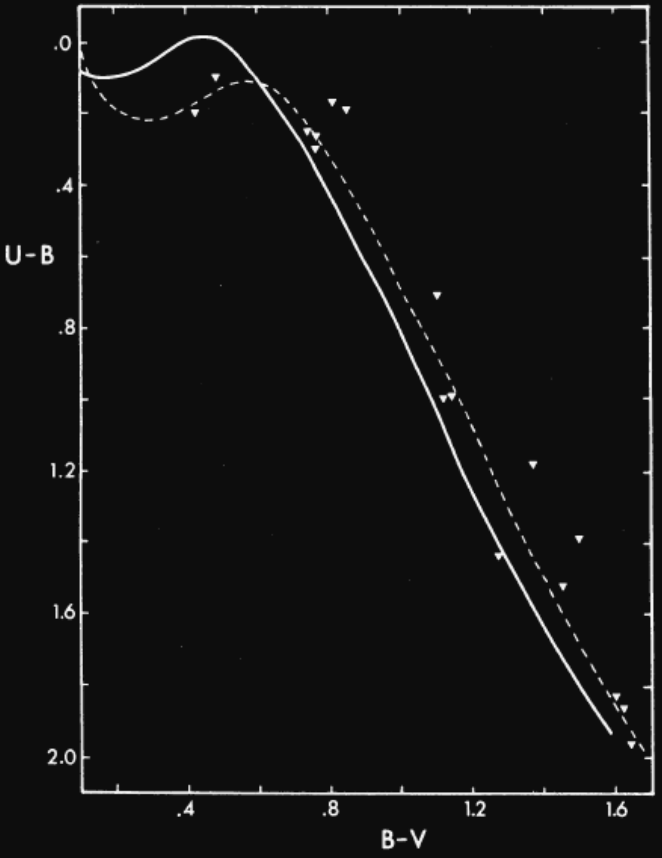
\includegraphics[width=0.72\textwidth]{grafico2.png}
\caption{\textbf{Mapas de Poincaré com interseção em $q_1 = 0$ com $E = 0,125$.}}
\end{figure}

Na Figura 2, são apresentados mais quatro mapas de Poincaré com a interseção ocorrendo em $q1 = 0$. Assim como na Figura 1, cada mapa é representado por pontos no plano cartesiano, com o eixo $x$ representando a variável $q_2$ e o eixo $y$ representando a variável $p_2$. Novamente, a cor dos pontos varia para diferenciar os diferentes mapas.

Esses mapas adicionais oferecem mais insights sobre as características do sistema Hénon-Heiles com a interseção em $q_1 = 0$. Ao comparar esses mapas com os anteriores, é possível analisar a sensibilidade do sistema às condições iniciais e identificar diferentes regimes dinâmicos. Nesse caso foi modificada apenas o valor da energia, e é possível perceber que as trajetórias aparentam ser bem mais caóticas nesses valores.

\begin{figure}[H]
\centering
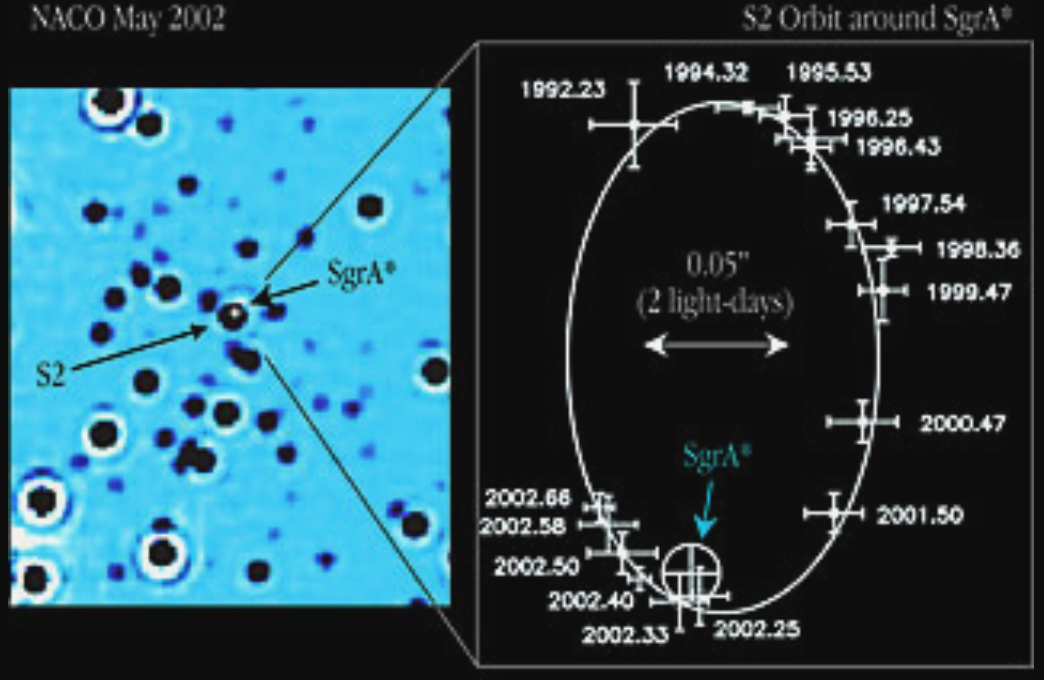
\includegraphics[width=1\textwidth]{grafico3.png}
\caption{\textbf{Curvas $q_1$, $p_1$, $q_2$ e $p_2$ em função do tempo - trajet. periódica com $E = 0,125$.}}
\end{figure}

Na Figura 3, foram plotadas as curvas das variáveis $q_1$, $p_1$, $q_2$ e $p_2$ em função do tempo, para uma condição inicial correspondente a uma trajetória periódica na seção de Poincaré com energia $E = 0,125$. Cada variável é representada em um sub-gráfico separado, como é possível observar.

A curva de $q_1$ em função do tempo (sub-gráfico superior esquerdo) mostra a evolução temporal da variável $q_1$. A curva de $p_1$ em função do tempo (sub-gráfico superior direito) mostra a evolução temporal da variável $p_1$. Da mesma forma, as curvas de $q_2$ e $p_2$ em função do tempo (sub-gráficos inferiores) mostram a evolução temporal das variáveis $q_2$ e $p_2$, respectivamente.

Essas curvas fornecem uma representação visual do comportamento da trajetória periódica no espaço de fase ao longo do tempo. É possível observar a periodicidade e a regularidade dessas curvas, indicando um movimento ordenado e previsível do sistema.



\begin{figure}[H]
\centering
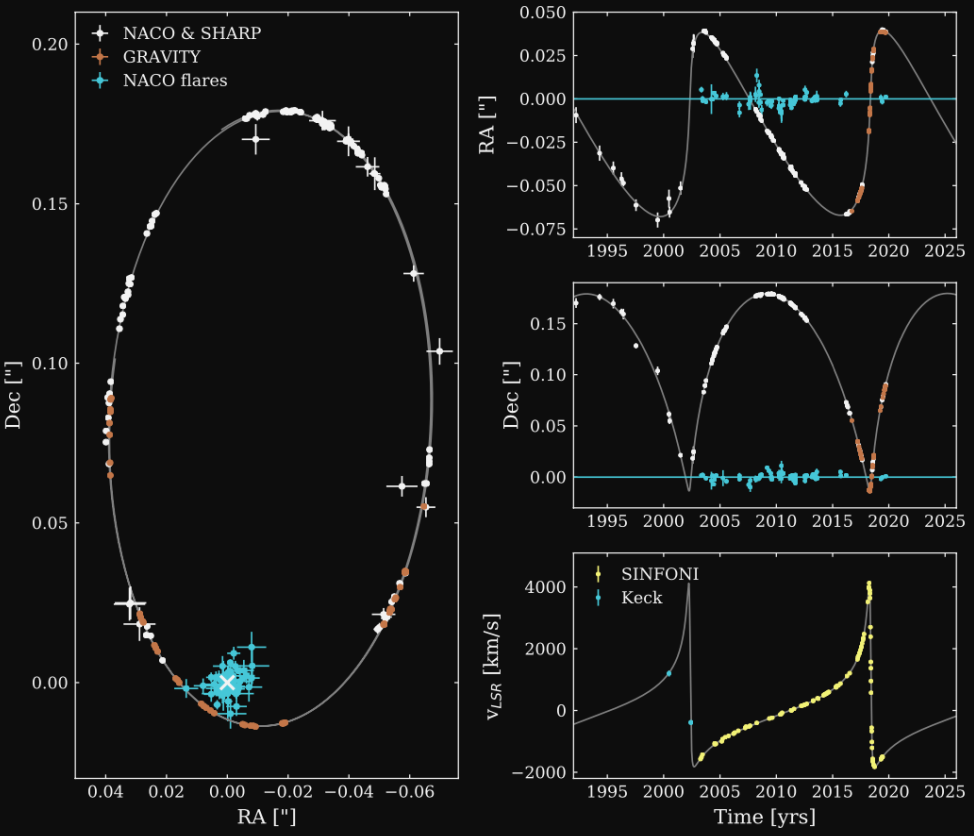
\includegraphics[width=1\textwidth]{grafico4.png}
\caption{\textbf{Curvas $q_1$, $p_1$, $q_2$ e $p_2$ em função do tempo - trajet. caótica com $E = 0,125$.}}
\end{figure}

Na Figura 4, de forma análoga à anterior, foram plotadas as curvas das variáveis $q_1$, $p_1$, $q_2$ e $p_2$ em função do tempo, mas desta vez para uma condição inicial correspondente a uma trajetória caótica na seção de Poincaré com energia $E = 0,125$. Cada variável é representada em um sub-gráfico separado, como é possível observar.

As curvas têm a mesma interpretação que na Figura 3, representando a evolução temporal das variáveis $q_1$, $p_1$, $q_2$ e $p_2$. No entanto, para uma trajetória caótica, espera-se que essas curvas sejam irregulares e imprevisíveis, sem um padrão claro ou período definido.

Ao analisar essas curvas, é possível perceber o comportamento caótico do sistema Hénon-Heiles. Pequenas variações nas condições iniciais podem levar a grandes diferenças nas trajetórias ao longo do tempo, caracterizando a sensibilidade do sistema às condições iniciais e a presença do caos determinístico.

Em conclusão, a análise da Hamiltoniana de Hénon-Heiles e a construção de seções de Poincaré oferecem uma abordagem abrangente para investigar os sistemas físicos não-lineares. Através da implementação computacional e da visualização gráfica, foi possível explorar as características dinâmicas, distinguir comportamentos regulares de caóticos e analisar a sensibilidade do sistema às condições iniciais. Esses resultados ampliam nosso conhecimento sobre os fenômenos estudados, fortalecendo a compreensão teórica e possibilitando a visualização dos resultados de forma acessível. O estudo da Hamiltoniana de Hénon-Heiles e das seções de Poincaré desempenha um papel crucial na compreensão de sistemas físicos complexos e na investigação de comportamentos dinâmicos não triviais.
\end{document}



